\chapter{Implementation and experimental setup}
\label{chap:dataset}
% This chapter will show the software and hardware used to perform the experiments described in \autoref{chap:experiments}.
In this chapter, we describe the experimental setup used to perform the experiments described in \autoref{chap:experiments}. We begin by showing the software and hardware that made this work possible. Then we describe the dataset used to train and test the models. Finally, we show and explain the metrics used to evaluate the models.

\section{Software}

    % The software tools used are: Pytorch, an open-source \acrfull{ml} Python framework used to build, train, and test the \acrshort{dl} models. Wandb \cite{wandb}, a dashboard used to collect and display all the metrics of the models. Scikit-learn is used to compute model metrics. Matplotlib and seaborn are used to generate charts.

    The project is developed in Python 3.9 and composed of multiple classes. A handful of libraries and frameworks are used to develop the code, namely:

    \begin{itemize}
        \item Pytorch \cite{pytorch}
        \item WandB \cite{wandb}
        \item Scikit-learn
        \item Albumentations
        \item Matplotlib and Seaborn
        \item Pandas
        \item Numpy
    \end{itemize}

    The final code is available on \href{https://github.com/aXhyra/Active-Learning-for-Visual-Anomaly-Detection-Applied-to-Mobile-Robots}{GitHub} and in \autoref{chap:code}.

    \subsection{Pytorch}
    Pytorch \cite{pytorch} is an open-source \acrfull{ml} Python framework used to build, train, and test the \acrshort{dl} models. This framework was originally developed by Meta, but now it is part of the Linux Foundation. It is a \acrfull{dl} framework that provides two high-level features:

    \begin{itemize}
        \item Numpy-like Tensor computation with strong GPU acceleration.
        \item Deep neural networks built on a tape-based autogradient system.
    \end{itemize}
    
    This framework is used as the base to develop, build, train and test the models used in this work.

    \subsection{WandB}
    Wandb \cite{wandb} is a dashboard used to collect and display all the metrics of the models. It is a tool that allows to track and visualize the training of the models. It is also used to compare the results of different models. 
    
    We use this library to keep track of model metrics during training, validation, and testing.

    \subsection{Scikit-learn}
    Scikit-learn is a Python library used to compute model metrics. It is a Python \acrfull{ml} library. It features various classification, regression and clustering algorithms. Some of which include support vector machines, random forests, and more. It is designed to interoperate with the Numpy and Scipy libraries.
    
    This library is used to compute the model test metrics, in our case the \acrfull{auc} score.
    
    \subsection{Albumentations}
    Albumentations \cite{albumentation} is a computer vision library used to perform \emph{data augmentation} in image datasets. This library is a part of the PyTorch ecosystem, it can be easilly integrated with the most used \acrshort{dl} frameworks.
    
    We use this library to perform data augmentation on the Hazards\&Robots dataset, Corridors scenario.
    
    \subsection{Matplotlib}
    Matplotlib is a Python library used to generate charts. It is a comprehensive library for creating static, animated, and interactive visualizations in Python.

    \subsection{Numpy}
    Numpy is a widely used Python library used to manipulate arrays. It is a core library for Python scientific computing. It contains among other things: a powerful N-dimensional array object (ndarray), sophisticated (broadcasting) functions, tools for integrating C/C++ and Fortran code, useful linear algebra, Fourier transform, and random number capabilities.
        
    Vectorization and broadcasting are two essential concepts in Numpy. Vectorization makes writing array operations easier by making loops and array indexing implicit. Broadcasting is a set of rules for applying binary functions (addition, subtraction, multiplication, \dots) on arrays of different sizes.
    
    The library provides a multidimensional array object named ndarray, various derived objects (such as masked arrays and matrices), and many routines for fast array operations, some of which include mathematical, logical, shape manipulation, sorting, selecting, I/O, discrete Fourier transforms, basic linear algebra, statistical operations, random simulation and more.

    The ndarray object is the core of the Numpy library. This object is a multidimensional array of homogeneous data types. It provides many operations written in C for improved performance. It is a fast and space-efficient multidimensional container for generic data.
    
    We use this library in conjunction with Pytorch and Scikit-learn to compute model metrics.
    
    \section{Hardware}
        \subsection{Workstation}
        The majority of experiments are conducted on a cluster available to \acrshort{idsia} intelligent robotics lab. The cluster has the following hardware:
        \begin{itemize}
            \item 4 Nvidia RTX 2080TI GPUs
            \item 128GB of ram
            \item 2 Intel(R) Xeon(R) Gold 5217 8-core, 16-threads CPUs
        \end{itemize}
        Model training uses only one GPU at a time.
        \\
        \\
        Some test experiments and initial model testing are conducted on a mobile workstation equipped with:
        \begin{itemize}
            \item Nvidia Quadro T2000 GPU
            \item 16GB of ram
            \item Intel(R) Core(TM) i7-9850H  CPU
        \end{itemize}

    % \begin{figure}[H]
    %     \centering
    %     \centerline{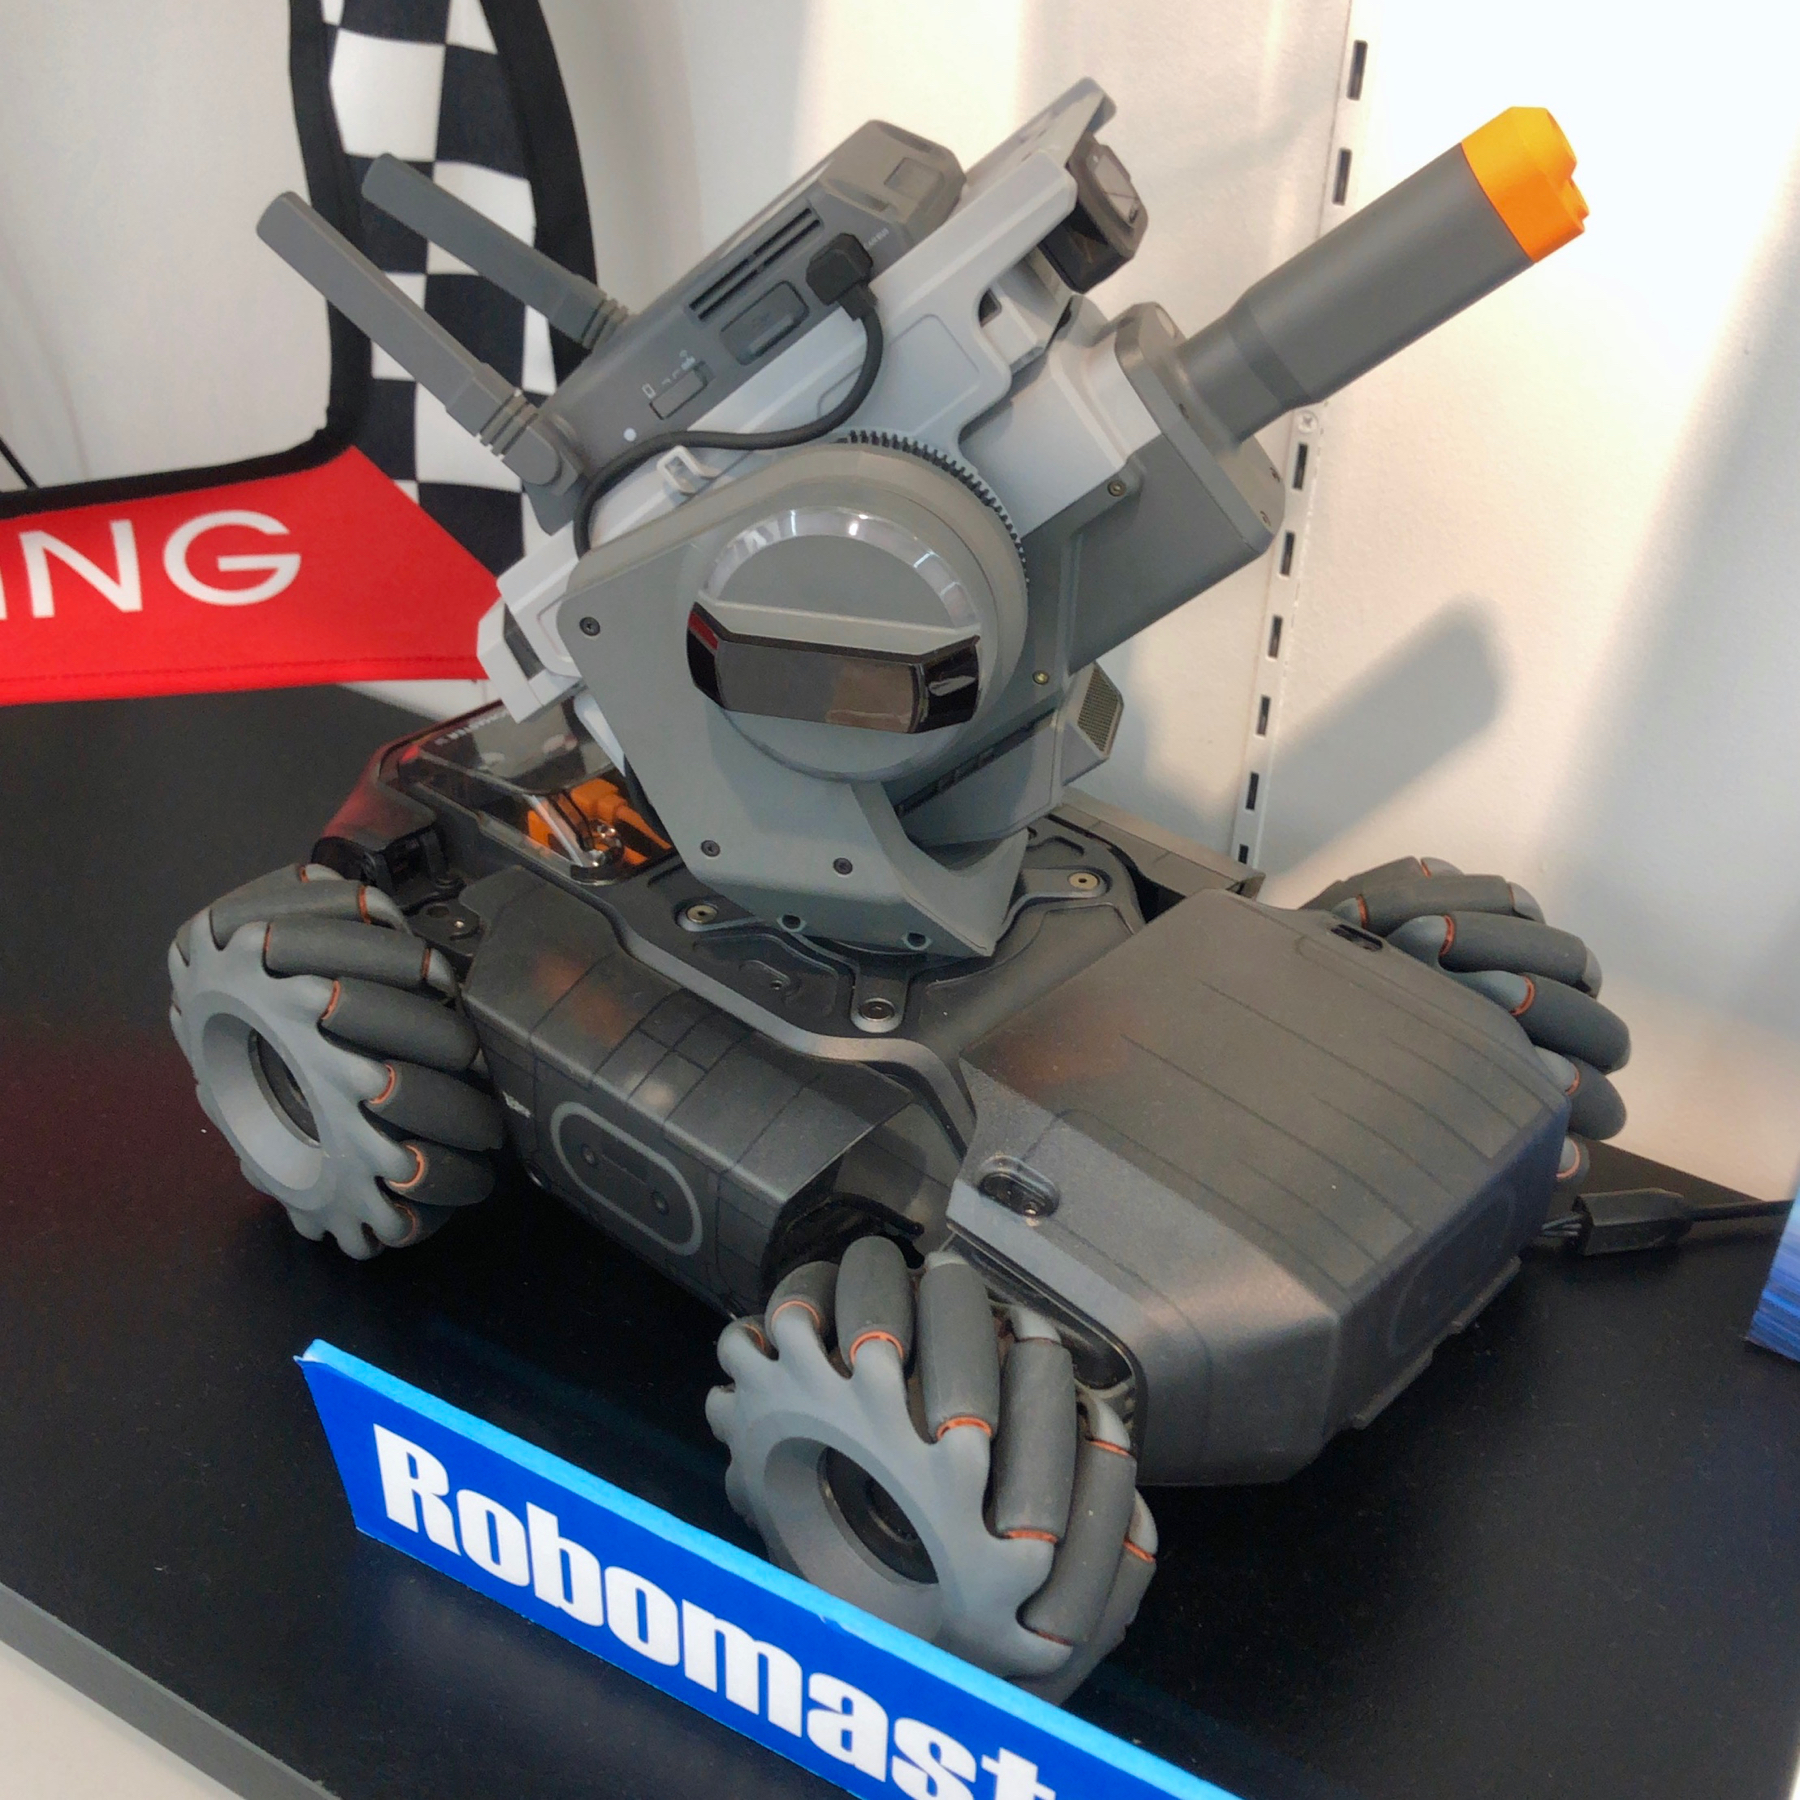
\includegraphics[width=\textwidth]{img/DJI_RoboMaster_S1.jpg}}
    %     \caption{Robomaster S1}
    %     \label{fig:env-ex}
    % \end{figure}
    
        \subsection{DJI Robomaster S1}
        \label{sub:robomaster}
        The robot used for this project is the DJI Robomaster S1 (\autoref{fig:robomaster}, \ref{fig:env-ex}), the first consumer-level ground robot of the company. It is named after the company's annual robot combat competition.
        
        The S1 is a remotely controlled, tank-like rover that can be operated in first-person view using Wi-Fi and an app on devices running Android, iOS, or Windows. The user has to assemble the robot out of the box from loose parts and learn to program it. It is intended to be an "advanced teaching robot" meant to teach kids how to code.

        \begin{figure}[htpb]
            \centering
            \centerline{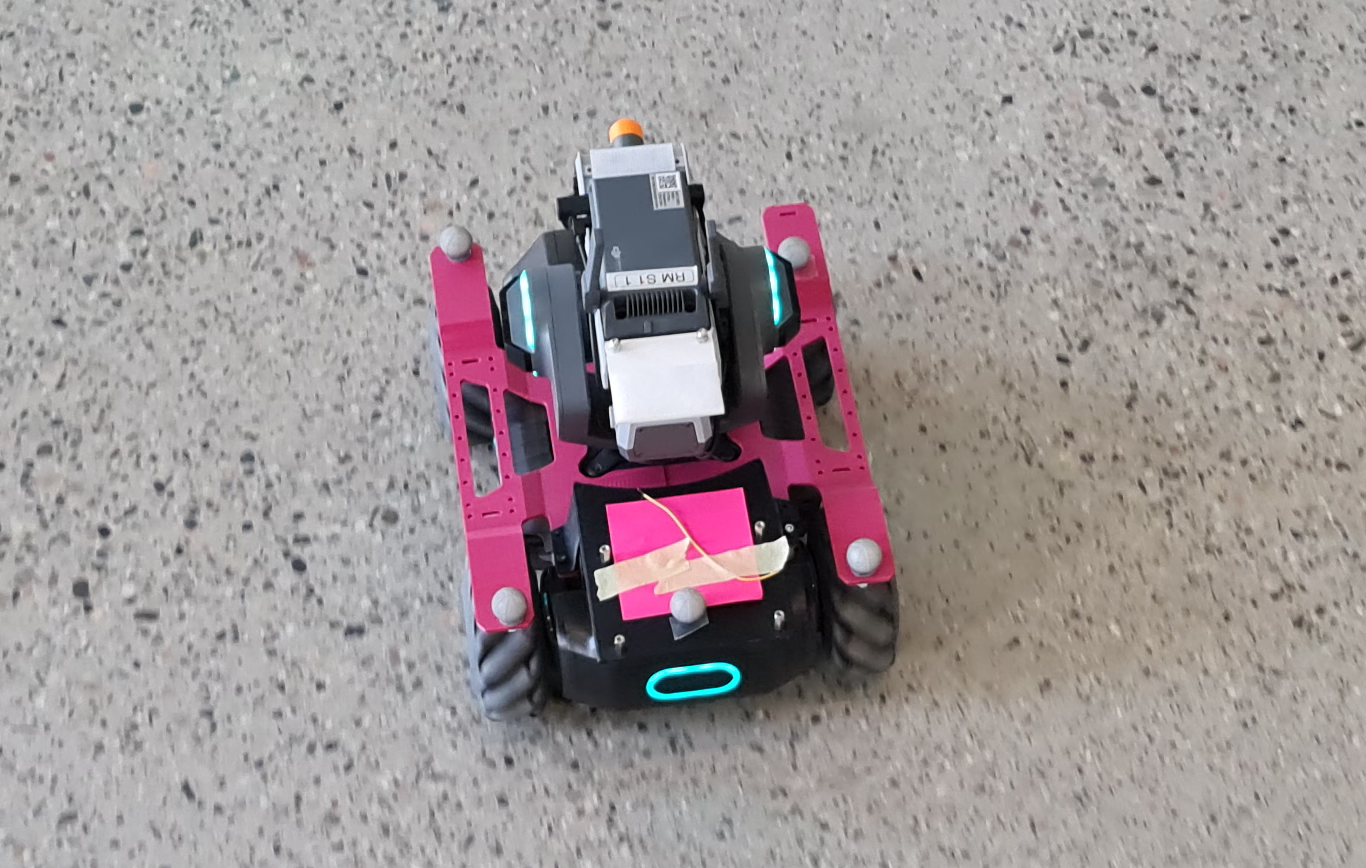
\includegraphics[width=\textwidth]{img/robomaster.png}}
            \caption{Robomaster S1, picture shot during data collection.}
            \label{fig:robomaster}
        \end{figure}
        
        \subsubsection{Hardware description}
            The Robomaster S1 is a ground robot capable of both indoor and outdoor drives. Thanks to its \emph{Mecanum wheels} \cite{ilon1975wheels} it can move in any direction. It can achieve a maximum speed of 13 km/h moving forwards, 9 km/h moving backward, and 10 km/h moving laterally.

            The robot comes with a 2400 mAh battery which lasts about 30 minutes when fully charged. A quick battery release system lets the user change an empty battery with a charged one in a matter of seconds.
            
            The robot is usually remote-controlled using the Robomaster app on a smartphone, tablet, or computer. The robot can be configured to act as an \acrfull{ap} or connect to a WLAN router. Depending on the connection type and the frequency used (the robot supports both 2.4 and 5 GHz networks) the operating range may vary from a minimum of 90m to a maximum of 300m.
            
            Once connected to the robot the app provides the live camera feed from the robot's camera, letting the user control it in first-person view.
            
            For the data collection phase, the robot is operated using the app and the videos are recorded to an onboard micro sd card.

            Both python and scratch official SDK is available for the robot. The python SDK is a wrapper around the Robomaster's \acrshort{api} and allows to control of the robot using python scripts. The robot can be also interfaced with \acrfull{ros} via an unofficial \acrshort{api} wrapper developed in \acrshort{idsia} \cite{JeromeRobomaster}.

            
            \subsubsection*{Camera}
                The Robomaster S1 comes with a 120° \acrshort{fov} 5 Megapixel camera capable of recording Full-HD video at 30 \acrshort{fps} with a maximum bitrate of 16Mbps. The camera is mounted on a 2-axis gimbal, which provides mechanical camera stabilization for Pitch and Yaw.
                
            \begin{figure}[H]
                \centering
                \centerline{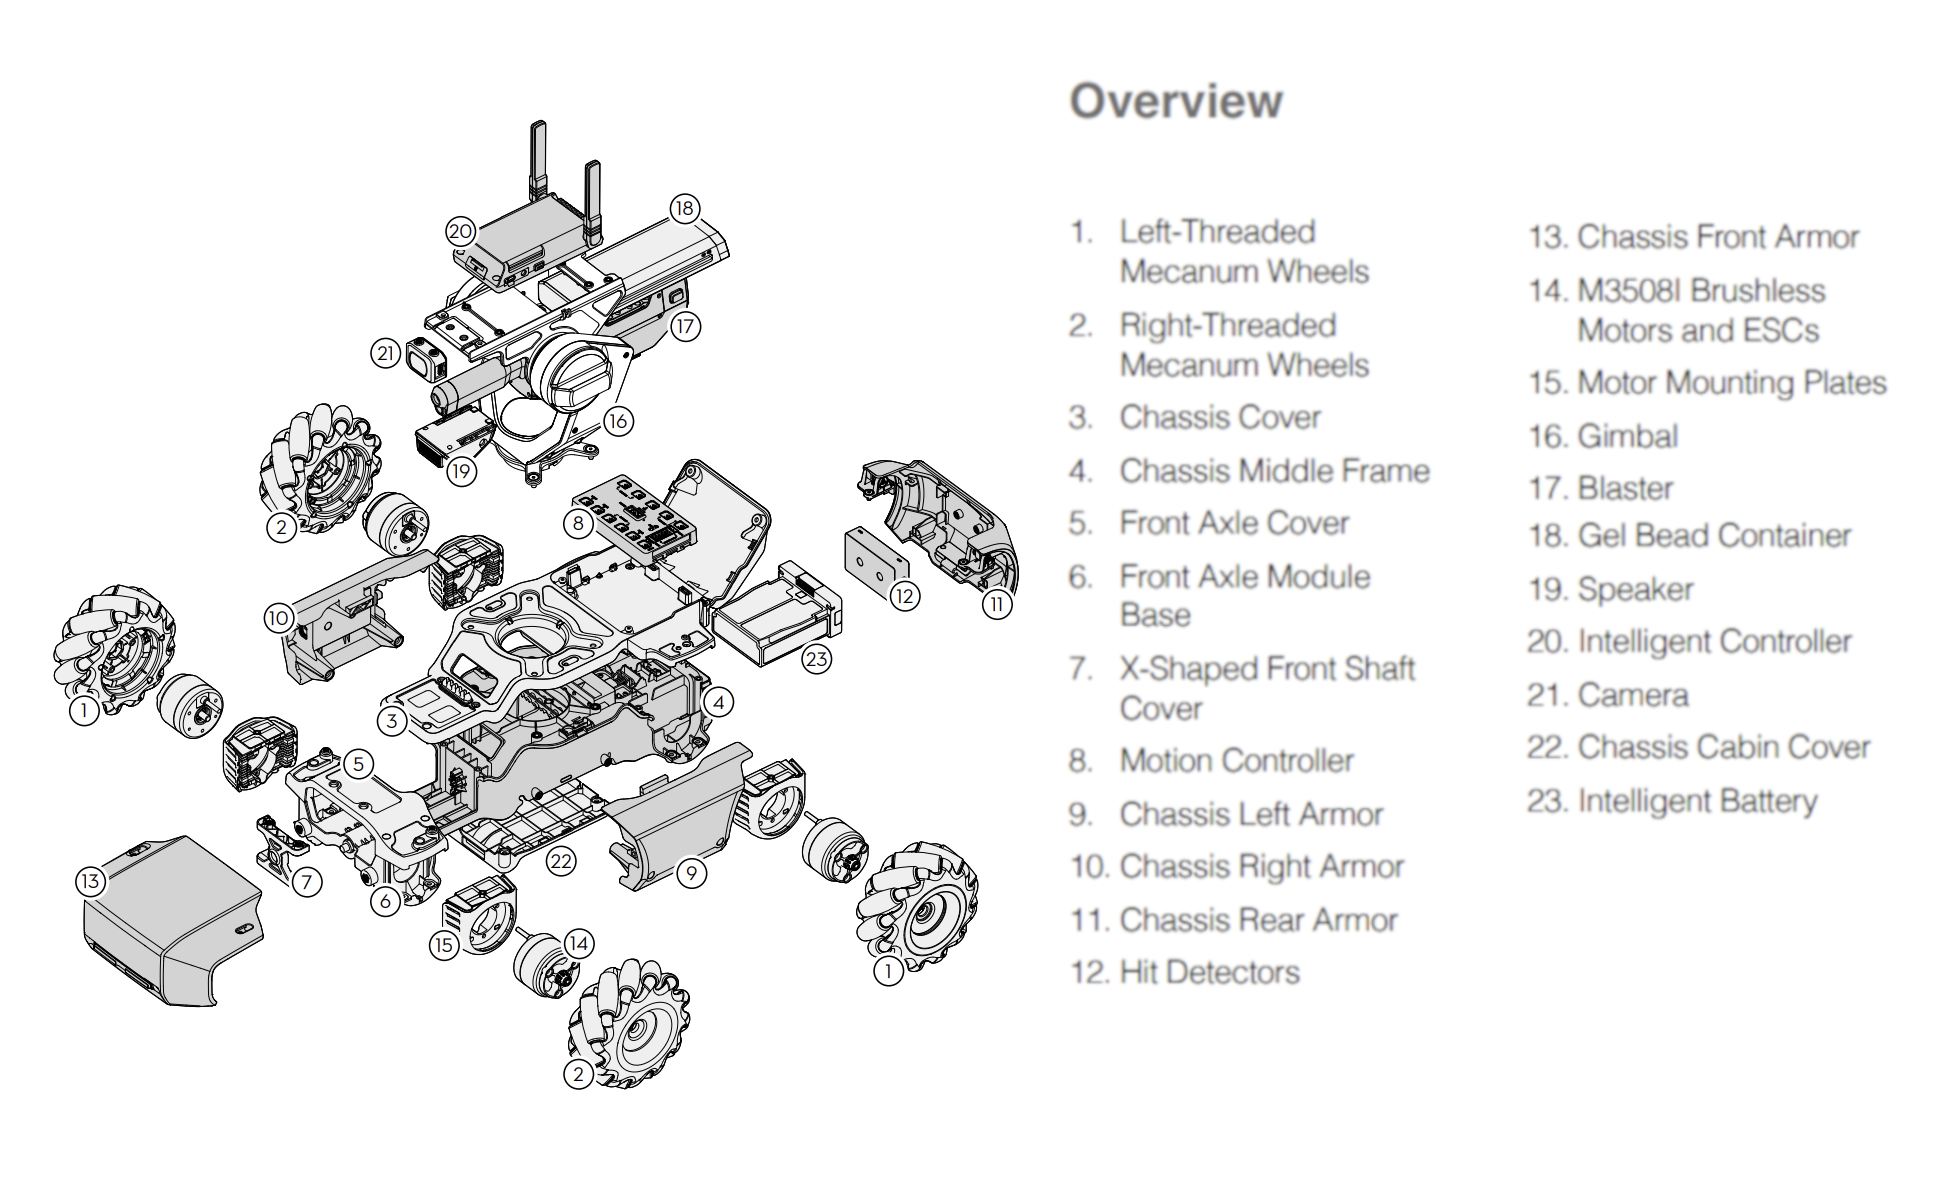
\includegraphics[width=\textwidth]{img/RM-exploded.png}}
                \caption{Robomaster S1, exploded-view from user manual with part names.}
                \label{fig:env-ex}
            \end{figure}
            
\section{Anomaly Detection model}
    
    The \acrshort{dl} model we use to solve the task of anomaly (shown in \autoref{tab:model}) is a \acrfull{cae} implemented in pytorch~\cite{pytorch}, inspired from the work done in \acrshort{idsia}~\cite{Idsia}.
    
    The encoder is a \acrfull{cnn} composed of 4 convolutional layers with dropout inserted after the second convolution and the third one.
    
    
    The network bottleneck is a Fully Connected Network. Its input layer receives the flattened output of the encoder. The \emph{hidden layer} has dimension \emph{16}, and the output layer has the same size as the input one ($64*64*3$ for the RoboMaster dataset, $28*28$ for MNIST).
    
    
    The decoder has the inverted structure of the encoder. It uses \emph{Transposed Convolutional} layers and dropout.
    
    The \emph{Reconstruction error} is computed as the \acrfull{mse} (\autoref{eq:mse}) between the input frame and the output of the autoencoder. This metric is used to check whether a frame is anomalous: the higher the error (anomaly score), the higher the probability the frame is anomalous.
    
    % The used model is a \acrfull{cae} implemented in PyTorch \cite{pytorch} with the following architecture:
    % The activation function used in each layer is the LeakyReLu \cite{maas2013rectifier} function, except for the encoder and decoder
    %     output layers, which use the sigmoid function.
    
        % Please add the following required packages to your document preamble:
        % \usepackage{graphicx}
        \begin{table}[!htpb]
        \centering
        \resizebox{\textwidth}{!}{%
        \begin{tabular}{lrllllr}
        \hline
        \multicolumn{3}{c}{\textbf{Layer}} &
           &
          \multicolumn{1}{c}{\textbf{Output Shape}} &
           &
          \multicolumn{1}{c}{\textbf{\begin{tabular}[c]{@{}c@{}}Number of\\ Parameters\end{tabular}}} \\ \hline
                    & \multicolumn{1}{l}{}           &                 &  &                 &  &        \\ \hline
        Autoencoder & \multicolumn{1}{l}{}           &                 &  &                 &  &        \\
        |-          & \multicolumn{2}{l}{ConvolutionalEncoder}         &  & [1, 2048]       &  &        \\
        |           & |-                             & Conv2d          &  & [1, 16, 26, 26] &  & 160    \\
        |           & |-                             & Conv2d          &  & [1, 32, 24, 24] &  & 4640   \\
        |           & |-                             & Dropout         &  & [1, 32, 24, 24] &  &        \\
        |           & |-                             & Conv2d          &  & [1, 64, 11, 11] &  & 18496  \\
        |           & |-                             & Dropout         &  & [1, 64, 11, 11] &  &        \\
        |           & |-                             & Conv2d          &  & [1, 128, 4, 4]  &  & 295040 \\
        |-          & \multicolumn{1}{l}{Bottleneck} &                 &  & [1, 128, 4, 4]  &  &        \\
        |           & |-                             & Linear          &  & [1, 64]         &  & 131136 \\
        |           & |-                             & Linear          &  & [1, 2048]       &  & 133120 \\
        |- &
          \multicolumn{1}{l}{ConvolutionalDecoder} &
           &
           &
          [1, 1, 28, 28] &
           &
           \\
        |           & |-                             & ConvTranspose2d &  & [1, 64, 12, 12] &  & 294976 \\
        |           & |-                             & ConvTranspose2d &  & [1, 32, 25, 25] &  & 18464  \\
        |           & |-                             & Dropout         &  & [1, 32, 25, 25] &  &        \\
        |           & |-                             & ConvTranspose2d &  & [1, 16, 27, 27] &  & 4624   \\
        |           & |-                             & Dropout         &  & [1, 16, 27, 27] &  &        \\
        |           & |-                             & ConvTranspose2d &  & [1, 1, 29, 29]  &  & 145    \\ \hline
                    & \multicolumn{1}{l}{}           &                 &  &                 &  &        \\ \hline
        \multicolumn{7}{l}{Total params: 900,801}                                                       \\
        \multicolumn{7}{l}{Trainable params: 900,801}                                                   \\
        \multicolumn{7}{l}{Non-trainable params: 0}                                                     \\
        \multicolumn{7}{l}{Total mult-adds (M): 67.51}                                                  \\ \hline
                    & \multicolumn{1}{l}{}           &                 &  &                 &  &        \\ \hline
        \multicolumn{7}{l}{Input size (MB): 0.00}                                                       \\
        \multicolumn{7}{l}{Forward/backward pass size (MB): 0.66}                                       \\
        \multicolumn{7}{l}{Params size (MB): 3.60}                                                      \\
        \multicolumn{7}{l}{Estimated Total Size (MB): 4.27}                                             \\ \hline
        \end{tabular}%
        }
        \caption{Model architecture}
        \label{tab:model}
        \end{table}
    
        The models are trained using the Adam optimizer \cite{kingma2014adam} with a learning rate of 1e-4 and random noise has been added to the images during training.
    
    
            % \begin{itemize}
            %     \item Encoder:
            %     \begin{itemize}
            %         \item Input layer BSZ x 1 x 28 x 28
            %         \item Convolutional layer 16 filters of size 3x3 with stride 1
            %         \item Convolutional layer 32 filters of size 3x3 with stride 1
            %         \item Convolutional layer 64 filters of size 3x3 with stride 2
            %         \item Convolutional layer 128 filters of size 6x6 with stride 2 and padding 1
            %         \item Output Fully-Connected bottleneck layer of size BSZ x 4
            %     \end{itemize}
            %     \item Decoder:
            %     \begin{itemize}
            %         \item Input layer of size BSZ x 4
            %         \item Fully-Connected layer of size BSZ x 128 x 4 x 4
            %         \item Deconvolutional layer 64 filters of size 6x6 with stride 2 and padding 1
            %         \item Deconvolutional layer 32 filters of size 3x3 with stride 2
            %         \item Deconvolutional layer 16 filters of size 3x3 with stride 1
            %         \item Output Deconvolutional layer of size BSZ x 1 x 28 x 28
            %     \end{itemize}
            % \end{itemize}
    

\section{Evaluation metrics}
    During the training phase, the model optimizes the \acrfull{mse} (\autoref{eq:mse}), with the \acrfull{mae} (\autoref{eq:mae}) being tracked as a side metric to check the performance. During the test phase, the \acrfull{auc} (\autoref{eq:auc}) metric is used to evaluate the model performance on the test set.
    

    Before introducing the metrics we first define the following terms:
    \begin{itemize}
        \item \textbf{TP} True Positive: the number of correctly classified positive samples;
        \item \textbf{TN} True Negative: the number of correctly classified negative samples;
        \item \textbf{FP} False Positive: the number of incorrectly classified positive samples;
        \item \textbf{FN} False Negative: the number of incorrectly classified negative samples.
    \end{itemize}

    \subsection{True Positive Rate (TPR)}
    The \acrfull{tpr} is defined as:
    \begin{equation}
        \text{TPR} = \frac{\text{TP}}{\text{TP} + \text{FN}}
    \end{equation}
    where $\text{TP}$ is the number of true positives and $\text{FN}$ is the number of false negatives.

    \subsection{False Positive Rate (FPR)}
    The \acrfull{fpr} is defined as:
    \begin{equation}
        \text{FPR} = \frac{\text{FP}}{\text{FP} + \text{TN}}
    \end{equation}
    where $\text{FP}$ is the number of false positives and $\text{TN}$ is the number of true negatives.

    \subsection{Area Under the Curve (AUC)}
    The \acrfull{auc} is a common metric used to evaluate the performance of binary classification models. It is defined as:
    \begin{equation}
        % \text{AUC} = \frac{1}{n} \sum_{i=1}^{n} \text{TPR}_i - \text{FPR}_i
        \text{AUC} = \int_0^1 \text{TPR}(\tau) - \text{FPR}(\tau) 
        \label{eq:auc}
    \end{equation}
    where $\tau$ is the threshold value. The \acrshort{auc} is a good metric to evaluate the performance of binary classification models.
    
    An \acrshort{auc} of 0.5 means that the model is performing as well as a random model, while a \acrshort{auc} of 1.0 means that the model is performing perfectly.
    In probabilistic terms, the \acrshort{auc} is the probability of predicting a sample from the positive class as positive.


\section{Datasets}
    The used datasets are MNIST \cite{lecun1998mnist}, a simple dataset used as \emph{proxy} that makes the model testing and debugging phase easier, and the Hazards\&Robots dataset, Corridors scenario~\cite{mantegazza2022outlier}.

    \subsubsection{MNIST}
     
        MNIST was adapted to the task of \acrshort{ad} by using a single class as normal, thus training the model on that class only.

    The MNIST (\autoref{fig:mnist}) dataset contains 60,000 training images and 10,000 test images of handwritten digits. Each image is a 28x28 grayscale image. The dataset is divided into 10 classes, one for each digit. The dataset is balanced, meaning that each class has the same number of samples.
    \begin{figure}[H]
        \centering
        \centerline{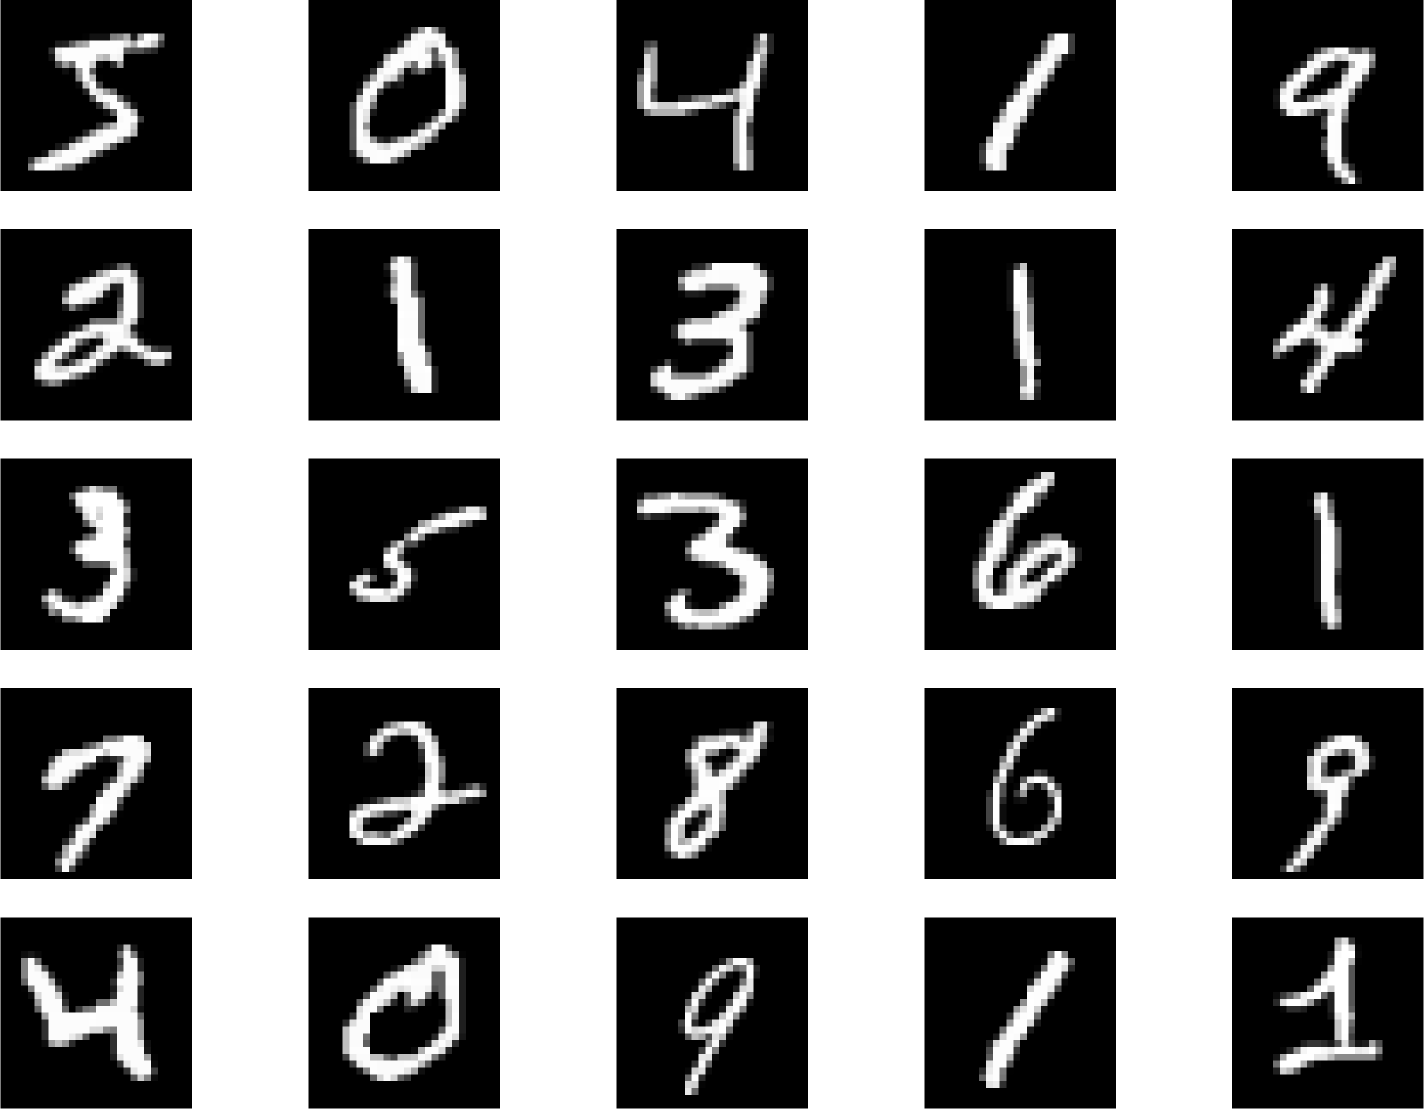
\includegraphics[width=\textwidth]{img/mnist_numbers.png}}
        \caption{Images from the MNIST dataset.}
        \label{fig:mnist}
    \end{figure}

    \subsubsection{Hazards\&Robots dataset}
    We extend the Hazards\&Robots dataset~\cite{mantegazza2022outlier}, corridors scenario (\autoref{fig:collected}) by collecting new frames using the ground robot described in \autoref{sub:robomaster}. The robot was driven around the campus of \acrfull{usi}, collecting images. The dataset contains 69,499 train images, 155,133 test images, and 4,163 images. Each sample is an RGB image with a resolution $64\times 64$.

    The dataset is structured into 21 classes, shown in \autoref{fig:collected} and explained in \autoref{chap:data-coll}.
    \begin{figure}[H]
        \centering
        \centerline{\includegraphics[width=\textwidth]{img/RM-Dataset.png}}
        \caption{Images from the Hazards\&Robots dataset.}
        \label{fig:collected}
    \end{figure}
    